\chapter{Capitulo de ejemplo}
\label{chap:ejemplo}
% Recursos bibliográficos para este capítulo (registrados en el preámbulo)
\begin{refsection}

Este capitulo deja una base minima para la memoria: texto, una imagen y un ejemplo de codigo.

\section{Imagen}

\begin{figure}[H]
    \centering
    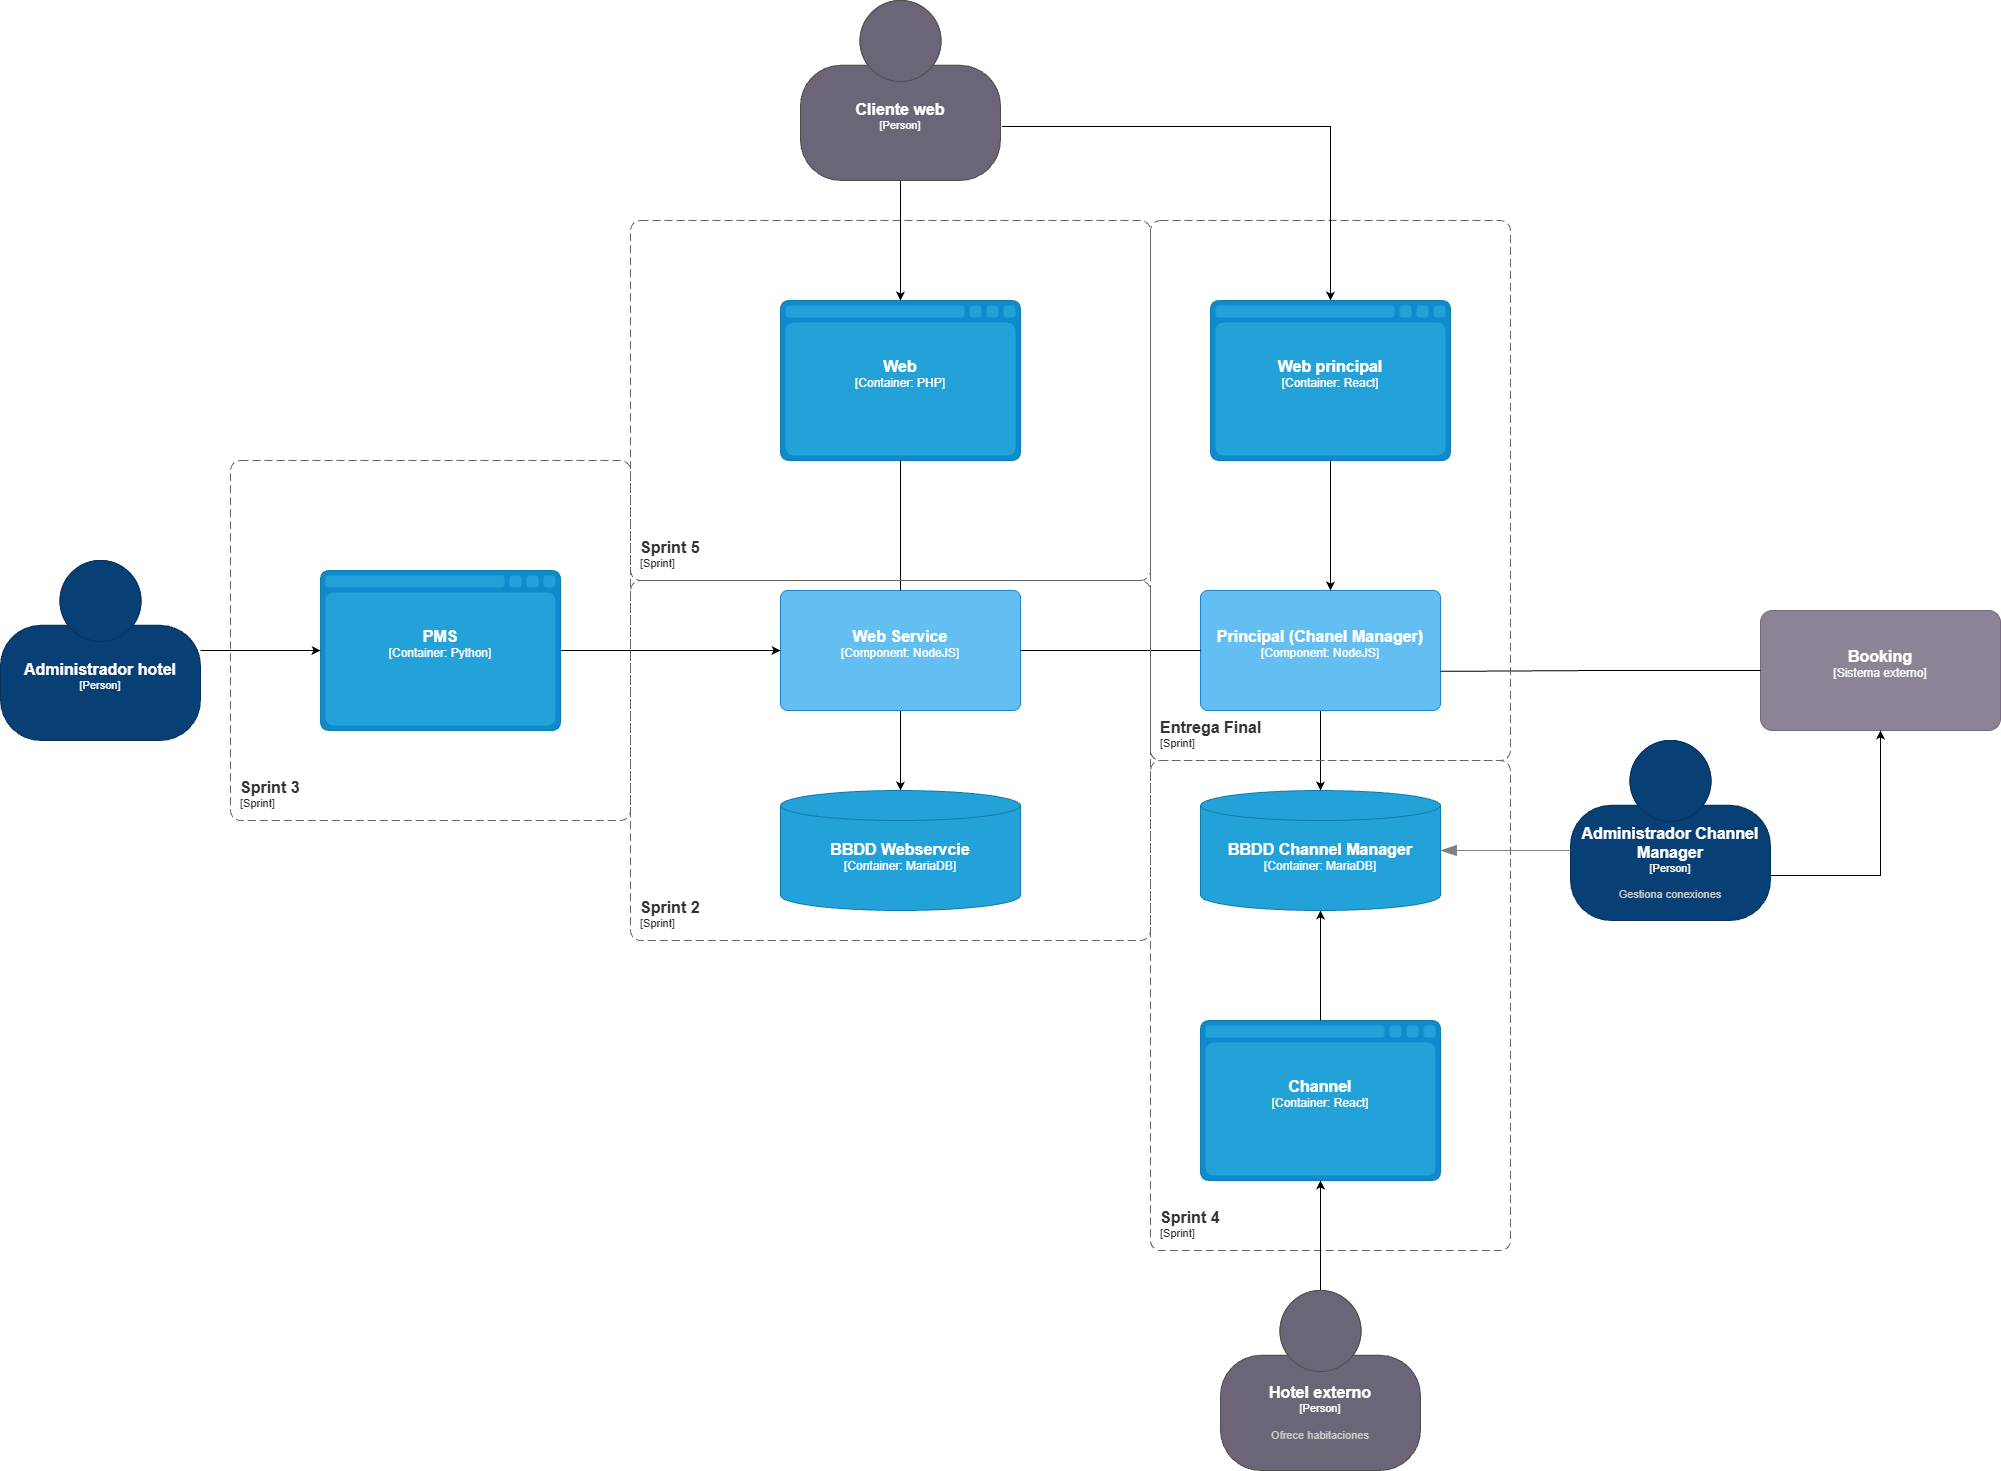
\includegraphics[width=0.8\textwidth]{images/content/arquitectura.png}
    \caption{Ejemplo de imagen reutilizada como referencia visual.}
    \label{fig:ejemplo_imagen}
\end{figure}

\section{Codigo}

\begin{lstlisting}[language=SQL, caption={Ejemplo de consulta sencilla}]
SELECT id, nombre
FROM hoteles
WHERE activo = 1;
\end{lstlisting}

\section{Texto}

Este bloque sirve como plantilla para ampliar la memoria manteniendo el mismo formato y la misma organizacion.

Un ejemplo de cita IEEE (número): como muestra \cite{knuth1984texbook}.

\subsection{Ejemplos de citas}

Citando un artículo de revista: \cite{smith2019fastalg}.

Citando un artículo de congreso: \cite{garcia2018confpaper}.

Citando una tesis: \cite{martinez2020thesis}.

Citando un recurso online/dataset: \cite{dataset2021open}.

Citando software: \cite{tool2022pkg}.

Varias citas a la vez: \cite{knuth1984texbook,smith2019fastalg,garcia2018confpaper}.

\printbibliography[heading=subbibliography]

\end{refsection}
